% makeindex < aebpro_man.idx > aebpro_man.ind
% http://www.acrotex.net/blog/?tag=mkstmpdad
\documentclass{article}
\usepackage[fleqn]{amsmath}
\usepackage[
    web={centertitlepage,designv,forcolorpaper,tight*,latextoc,pro},
    eforms,
%    linktoattachments,
%    attachments={../aeb_pro.dtx},
%    uselayers,
    aebxmp
]{aeb_pro}
\usepackage{aeb_mlink}
\usepackage{aeb_dad}
\usepackage{picins}

\usepackage{graphicx,array}
%\usepackage{myriadpro}
\usepackage[altbullet]{lucidbry}

%\usepackage{makeidx}
%\makeindex
\usepackage{acroman}

\usepackage[active]{srcltx}

\urlstyle{rm}
\def\pkg{\textsf}
\let\app\textsf
\let\uif\textsf
\def\meta#1{\textit{\texttt{#1}}}
\newdimen\aebdimen \aebdimen6pt %\partopsep \advance\aebdimen\partopsep
\renewcommand\bVerb[1][]{\begingroup#1\vskip\aebdimen\parindent0pt}%
\def\eVerb{\vskip\aebdimen\endgroup\noindent}

\def\darg#1{\texttt{\{#1\}}}
\def\takeMeasure{\bgroup\obeyspaces\takeMeasurei}
\def\takeMeasurei#1{\global\setbox\webtempboxi\hbox{\ttfamily#1}\egroup}
\def\bxSize{\wd\webtempboxi+2\fboxsep+2\fboxrule}

% The mkstmpdad Bundle: Using the mkstmp_pro Package to Create Custom
% Stamps, and Using the aeb_dad Package to Create Drag and Drop Matching

%\def\tutpath{doc/tutorial}
%\def\tutpathi{tutorial}

\DeclareDocInfo
{
    university={\AcroTeX.Net},
    title={\texorpdfstring{\huge}{}The \pkg{mkstmpdad} Bundle\texorpdfstring{\\[8pt]}{: }%
        \texorpdfstring{\Large}{}Using the \pkg{mkstmp\_pro} Package\texorpdfstring{\\}{ }%
        to Create Custom Stamps\texorpdfstring{\\[4pt]and\\[4pt]}{, and }%
        Using the \pkg{aeb\_dad} Package\texorpdfstring{\\}{ }%
        to Create Drag and Drop Matching
    },
    author={D. P. Story},
    email={dpstory@acrotex.net},
    subject=Documentation for the mkstmpdad bundle,
    talksite={\url{www.acrotex.net}},
    version={2016/10/26},
    Keywords={LaTeX,PDF,Stamps,drag and drop game},
    copyrightStatus=True,
    copyrightNotice={Copyright (C) \the\year, D. P. Story},
    copyrightInfoURL={http://www.acrotex.net}
}

\versionLabel{Bundle dated: }

\def\dps{$\hbox{$\mathfrak D$\kern-.3em\hbox{$\mathfrak P$}%
   \kern-.6em \hbox{$\mathcal S$}}$}

\universityLayout{fontsize=Large}
\titleLayout{fontsize=LARGE}
\authorLayout{fontsize=Large}
\tocLayout{fontsize=Large,color=aeb}
\sectionLayout{indent=-62.5pt,fontsize=large,color=aeb}
\subsectionLayout{indent=-31.25pt,color=aeb}
\subsubsectionLayout{indent=0pt,color=aeb}
\subsubDefaultDing{\texorpdfstring{$\bullet$}{\textrm\textbullet}}

\makeatletter
\renewcommand{\makeinlinetitle}
{%
    \begingroup\parskip0pt\parindent0pt
    \par\vspace*{6pt}
    \noindent\makebox[\linewidth][c]{\bfseries
    \color{\webuniversity@color}\webuniversity}\par\kern6pt\noindent
    \makebox[\linewidth][c]{\parbox[c]{.75\linewidth}{\centering
    \bfseries\color{\webtitle@color}\webtitle}}\par\kern12pt
    \noindent\parbox{\linewidth}{\scriptsize
        \web@copyright\space\the\year\hfill\thewebemail\\
        \@date\hfill\@ifundefined{aeb@talksite}{\webversion}
            {\ifx\aeb@talksite\@empty\webversion
              \else\aeb@talksite\fi}%
        }\par
    \noindent\makebox[\linewidth]{\rule{.67\linewidth}{.4pt}}%
    \par\endgroup
}
\renewcommand{\paragraph}
    {\@startsection{paragraph}{4}{0pt}{6pt}{-3pt}
    {\normalfont\normalsize\bfseries}}
\renewcommand{\subparagraph}
    {\@startsection{subparagraph}{5}{\parindent}{6pt}{-3pt}%
    {\normalfont\normalsize\bfseries}}

\makeatother

%\pagestyle{empty}
%\parindent0pt\parskip\medskipamount\setlength{\marginparsep}{4pt}


\chngDocObjectTo{\newDO}{doc}
\begin{docassembly}
var titleOfManual="The mkstmpdad Bundle";
var manualfilename="Manual_BG_Print_dad.pdf";
var manualtemplate="Manual_BG_Green.pdf"; // Blue, Green, Brown
var _pathToBlank="C:/Users/Public/Documents/ManualBGs/"+manualtemplate;
var doc;
var buildIt=false;
if ( buildIt ) {
    console.println("Creating new " + manualfilename + " file.");
    doc = \appopenDoc({cPath: _pathToBlank, bHidden: true});
    var _path=this.path;
    var pos=_path.lastIndexOf("/");
    _path=_path.substring(0,pos)+"/"+manualfilename;
    \docSaveAs\newDO ({ cPath: _path });
    doc.closeDoc();
    doc = \appopenDoc({cPath: manualfilename, oDoc:this, bHidden: true});
    f=doc.getField("ManualTitle");
    f.value=titleOfManual;
    doc.flattenPages();
    \docSaveAs\newDO({ cPath: manualfilename });
    doc.closeDoc();
} else {
    console.println("Using the current "+manualfilename+" file.");
}
var _path=this.path;
var pos=_path.lastIndexOf("/");
_path=_path.substring(0,pos)+"/"+manualfilename;
\addWatermarkFromFile({
    bOnTop:false,
    bOnPrint:false,
    cDIPath:_path
});
\executeSave();
\end{docassembly}
\begin{document}

\maketitle

\selectColors{linkColor=black}
\tableofcontents
\selectColors{linkColor=webgreen}

\section{Introduction}

This bundle consists of two related {\LaTeX} packages:
\begin{quote}
\begin{description}
    \item \pkg{mkstmp\_pro} is used to create stamps for display in
        \app{Adobe Acrobat} or \app{Adobe Reader}. \app{Adobe Acrobat}
        (and \app{Adobe Distiller}) are required to produce these stamps.
        The package requires \pkg{aeb\_pro}
        (\href{http://ctan.org/pkg/aeb-pro}{pkg/aeb-pro}), for it uses
        the \texttt{docassembly} environment to create the stamp file.

        The contents of the stamp file appears in the
        Comment panel, under the Add Stamp tool. A stamp
        can be dragged and dropped into a PDF document and a comment
        can be attached to it.

    \item \pkg{aeb\_dad} is an application to \pkg{mkstmp\_pro} and
        requires the \pkg{annot\_pro} package
        (\href{http://ctan.org/pkg/annot-pro}{pkg/annot-pro}). The
        \pkg{aeb\_dad} package is used to create a ``matching'' game, in
        which the user drags a stamp and drops it into a target region.
        Underlying JavaScript then determines whether the user has
        dropped the stamp in the correct region or not. This is as close
        to a drag and drop feature that you can get using Adobe PDF
        (without writing a plugin).
\end{description}
\end{quote}
The matching ``game'' created by the \pkg{aeb\_dad} package works for users
that have \app{Adobe Acrobat}, but the big news here is that it works also
for users of \app{Adobe Reader XI}! In the version~11 release, \app{Adobe
Reader} is now able to fill in forms and save and to provide access to all
comment features without requiring Reader Extended PDF;\footnote{This only
applies to non-XFA documents. XFA still requires Reader Extensions to save
filled in forms.} however, Adobe has dropped its support for browser-based
commenting, so functionality is limited from within a browser.

For more information on stamps, I recommend the book \emph{All About PDF Stamps,
In Acrobat \& Paperless Workflows}, by Thom Parker. See Thom's web site
\textbf{WindJack Solutions} at \url{windjack.com}.

\section{The \texorpdfstring{\pkg{mkstmp\_pro}}{mkstmp\_pro} Package}

The \pkg{mkstmp\_pro} enables the user of \app{Acrobat Pro} to
\textit{conveniently} create custom stamps.

\subsection{Requirements and Installation}

\pkg{mkstmp\_pro} requires \pkg{aeb\_pro} dated 2012/11/09 or later; in
particular, there has been a change to the \texttt{aeb\_pro.js} file, so
this new file must be installed, following the steps described in the
\pkg{aeb\_pro} manual.

As for the installation of \pkg{mkstmp\_pro}, if not automatically installed
by a {\TeX} system, just copy \texttt{mkstmp\_pro.sty} into a folder named
\texttt{mkstmpdad}. If appropriate, refresh the filename database of your
{\TeX} system.

\subparagraph*{Examples and Documentation.} Unzip \texttt{mkstmpdad.zip}
anywhere you want, outside the {\LaTeX} search path. The \textsf{ZIP} file will
create a folder named \texttt{mkstmpdad}, containing program files, and
folders \texttt{doc} and \texttt{examples}.

\subsection{Testing the system}

The \pkg{mkstmp\_pro} package comes with an example file,
\texttt{uspres\_stamps.tex}, which is found in the \texttt{mkstmpdad/\penalty0
examples/\penalty0mkstmp\_pro} folder. Accompanying this file is
\texttt{uspres.pdf}, found in the \texttt{images} subfolder.

The verbatim listing of \texttt{uspres\_stamps.tex} is given below.
\begin{Verbatim}[numbers=left,xleftmargin=20pt]
\documentclass{article}
\usepackage[web=designi]{aeb_pro}
\usepackage{mkstmp_pro}
\pagestyle{empty}

\title{U. S. Presidents Stamps}
\author{D. P. Story}

\setStampPath{C:/Users/Public/Documents/%
    My TeX Files/tex/latex/aeb/aebpro/mkstmpdad/%
    examples/mkstmp_pro/images/uspres.pdf}
\makeStamps{%
    {name=George Washington,page=0}
    {name=John Adams,page=1}
    {name=Thomas Jefferson,page=4}
    {name=James Madison,page=3}
    {name=John Quincy Adams,page=2}
}
\begin{docassembly}
\insertPreDocAssembly
\end{docassembly}

\begin{document}
\null\vfil
\begin{center}
\huge\sffamily\bfseries U. S. Presidents Stamps
\end{center}
\vfil
\end{document}
\end{Verbatim}
Before you can compile this file, you must edit lines~(9)--(10) to match
the path to the \texttt{examples} folder on your computer and save the
changes. Follow the steps outlined in the next paragraph, in these general
instructions, \ameta{my\_stamps} refers to the demo stamp file
\texttt{uspres\_stamps}.

\paragraph*{Procedure to create stamps.} The following are the steps for creating a stamp
file, \ameta{my\_stamps}.
\begin{enumerate}
\item \textbf{Create the Stamp file.} Now, {\LaTeX}
    \texttt{\ameta{my\_stamps}.tex}, convert the \textsf{DVI} to
    \textsf{PS} using \app{dvips}, then convert to PDF using
    \app{Adobe Distiller}. If all works out, the file
    \texttt{\ameta{my\_stamps}.pdf} is produced. When the file first opens
    in \app{Acrobat} after distillation, there are document assembly
    methods that import the images of the presidents into the newly
    created file. Give it a second or two for the process to complete
    before saving \texttt{\ameta{my\_stamps}.pdf}.

\item \textbf{Move the Stamp file.} After the stamp file is created,
    you need to move it to the stamp folder, where \app{Acrobat} expects it
    to be. To find this location, start \app{Acrobat} and open the
    JavaScript Debugger Window (\texttt{Ctrl+J}/\texttt{Cmd+J}), and
    type in the following line of code,
\begin{Verbatim}[xleftmargin=20pt]
app.getPath("user","stamps");
\end{Verbatim}
Place your cursor on this line and press
\uif{Ctrl+Enter}/\penalty0\uif{Cmd+Enter} (or just use the \uif{Enter} key
on the keypad). \app{Acrobat} will execute this line and return the path to
the user stamp folder. Navigate to this folder, and copy (or move)
\texttt{\ameta{my\_stamps}.pdf} to this folder.

\item Restart \app{Acrobat}.

\item\label{useannotpro} On restart, your newly installed stamps should be
    visible: Open the \uif{Comment} panel of \app{Acrobat}, and
    select the \uif{Add Stamp} tool.
\end{enumerate}
\bgroup
\parpic(50bp,50bp){\annotpro[subject={AcroTeX makes stamps},title={D. P.
Story},type=stamp,name=\#DPStory]{AcroTeX Rocks!}}
If you built and installed the \texttt{uspres\_stamp.pdf} file correctly,
\marginpar{\parbox[t]{40pt}{\vskip-.6\baselineskip\noindent\kern0pt
\annotpro[width=40bp,subject={AcroTeX makes stamps},title={D. P.
Story},type=stamp,name=\#George Washington]{You can use your stamps
through the user interface of Acrobat, or reference them with the
annot\_pro package!\n\n So says George Washington!}}}
you can use your stamps through the user interface of \app{Acrobat}, or
reference them with the \pkg{annot\_pro} package, as I did here (see the
comments of George Washington in the margin).\par\egroup

\begin{figure}[htb]\centering
\includegraphics[width=.33\linewidth]{graphics/comment_pane}
\caption{Stamp tool}\label{stamptool}
\end{figure}

\ding{228} To use stamps through the user interface of \app{Acrobat}:
\begin{itemize}
\item For \app{Acrobat 9} or earlier, select \uif{Comments > Show Comments
    \& Markup}. The Stamp tool can be seen on this toolbar. For
    \app{Acrobat~10} and later, select the \uif{Comment} panel on the
    right, again, the \uif{Stamp} tool is revealed. Figure~\ref{stamptool},
    page~\pageref{stamptool}, show the stamp tool, with \textbf{U.S.
    Presidents Stamps} selected.\footnote{The user-interface of
    \app{Acrobat} is ever changing.}
\item Select a stamp, click on it, and bring your mouse back over the
    document. An image of the stamp should appear. Place it by
    left-clicking.
\item Double click on the stamp to open the associated Pop-Up Note,
    used to associate a note with the stamp.
\end{itemize}

\subsection{The details}

A PDF file is used to create a stamp file. Each page that contains an
image for a stamp must be a \emph{page template} for that image to be
recognized as a stamp. A page template has an associated \emph{name} that is used
as the \emph{name} of the stamp, as can be seen through the user interface. The
stamps that appear in a stamp file are listed under that \textit{title} of the
stamp file in the Stamp tool menu, listing all available stamps, see
Figure~\ref{stamptool}, page~\pageref{stamptool}.

In light of the above paragraph describing the essentials of stamps, let's
go through the listing of \texttt{uspres\_stamps.tex}, which we'll
reproduce on this page.

%-62.5pt-31.25pt

\medskip

\def\Wdth{3.2in}
\hspace*{-62.5pt}\begin{minipage}[t]{\Wdth}\kern0pt
\begin{Verbatim}[numbers=left,xleftmargin=20pt,fontsize=\small]
\documentclass{article}
\usepackage[web=designi]{aeb_pro}
\usepackage{mkstmp_pro}
\pagestyle{empty}

\title{U. S. Presidents Stamps}
\author{D. P. Story}

\setStampPath{C:/Users/Public/Documents/%
 My TeX Files/tex/latex/aeb/aebpro/%
 mkstmpdad/examples/mkstmp_pro/images/%
 uspres.pdf}

\makeStamps{%
  {name=George Washington,page=0}
  {name=John Adams,page=1}
  {name=Thomas Jefferson,page=4}
  {name=James Madison,page=3}
  {name=John Quincy Adams,page=2}
}

\begin{docassembly}
\insertPreDocAssembly
\end{docassembly}

\begin{document}
\null\vfil
\begin{center}\huge\sffamily\bfseries
U. S. Presidents Stamps
\end{center}
\vfil
\end{document}
\end{Verbatim}
\end{minipage}\hfill
\begin{minipage}[t]{\linewidth+62.5pt-\Wdth-20pt}
Line~(2) we use the \textsf{aeb\_pro} package, which defines the
\texttt{docassembly} environment, seen in lines~(21)--(23). Line~(3)
inputs \textsf{mkstmp\_pro}, this package.
\vskip6pt
On line~(6) we title this document, the title appears in the Stamp menu, as
seen in Figure~\ref{stamptool} of page~\pageref{stamptool}.
\vskip6pt
The \cs{setStampPath} command is defined in this package to point to the
file containing the images to be made into stamps, call this the
\emph{images file}. It is an absolute path.
\vskip6pt
The \cs{makeStamps} command is the one that describes the images to be
imported into the document as stamps. Details are found below; in this example we specify
a \texttt{name} for the stamp, and the \texttt{page} on which this stamp
is to be found in the images file.
\vskip6pt
The \texttt{docassembly} environment, lines~(21)--(23), encloses the command
\cs{in\-sert\-Pre\-Doc\-As\-sem\-bly}. These two are defined in \textsf{aeb\_pro}, but
\textsf{mkstmp\_pro} modifies \cs{in\-sert\-Pre\-Doc\-As\-sem\-bly} to import and name
the images.
\vskip6pt
This content of the actual document is listed in lines~(26)-(30). No DVI
file is produced unless there is content. Here, we have a
simple title page.
\end{minipage}

\subsubsection{Commands of \texorpdfstring{\pkg{mkstmp\_pro}}{mkstmp\_pro}}

The \textsf{mkstmp\_pro} only defines two commands, \cs{setStampPath} and
\cs{makeStamps}.
\begin{itemize}
    \item \cs{setStampPath\{\ameta{absolute\_path}\}} defines the absolute path to
    the images file, the file that contains the images to be imported into
    the stamp file and used as stamps.
    \item \cs{makeStamps} takes a single argument that describes the images
    to be imported. The syntax is,
\begin{Verbatim}[numbers=left,xleftmargin=20pt,commandchars=!()]
\makeStamps{%
    {name=!meta(name!SUB1),page=!meta(page!SUB1)}
    {name=!meta(name!SUB2),page=!meta(page!SUB2)}
    ...
    {name=!meta(name!SUB(n)),page=!meta(page!SUB(n))}
}
\end{Verbatim}
The images will appear in the stamp file in the same order they are
listed. The value of the \texttt{name} key is the name to be associated
with the stamp. The value of the \texttt{page} key is the page that this
image is found on in the \emph{image} file. (Notice that in the verbatim
listing, the images are not imported in the same order they are listed in
the images file.) There is another key, not shown above, called
\texttt{path}. In theory, you can import an image in another file,
different from the one declared by \cs{setStampPath}. It is perhaps best
to have all images in a single file, however.
\end{itemize}

\subsection{The \textsf{mkstmp\_pro} workflow}

The workflow comes in two steps, prepare an \emph{images file}, create and install
the \emph{stamp file}.

\subsubsection{The images file}

The \pkg{mkstmp\_pro} package requires an \emph{images file}, a file
containing all the images to be made into stamps in the stamp file.
For the \texttt{uspres\_stamps.tex} file, the images file is
\texttt{uspres.pdf}, as seen at the end the absolute path declared by
\cs{setStampPath}.


Creating an images file is easy, given that you are using \app{Acrobat}.
Combining files into a single PDF is accomplished by opening \app{Acrobat}
and selecting \uif{Combine Files} into PDF from the menu or toolbar. Now the
good folks have moved things around over the years, so this features can
appear in diverse location depending on the version you are using. Your
\app{Acrobat} may have a Create button on the toolbar, as seen in
Figure~\ref{combine}.\footnote{Version~9 of \app{Acrobat} has a Create
button, but the feature here is now called Merge Files into a Single PDF.
It is also found under \uif{File > Combine}.}

\begin{figure}[htb]
\begin{center}
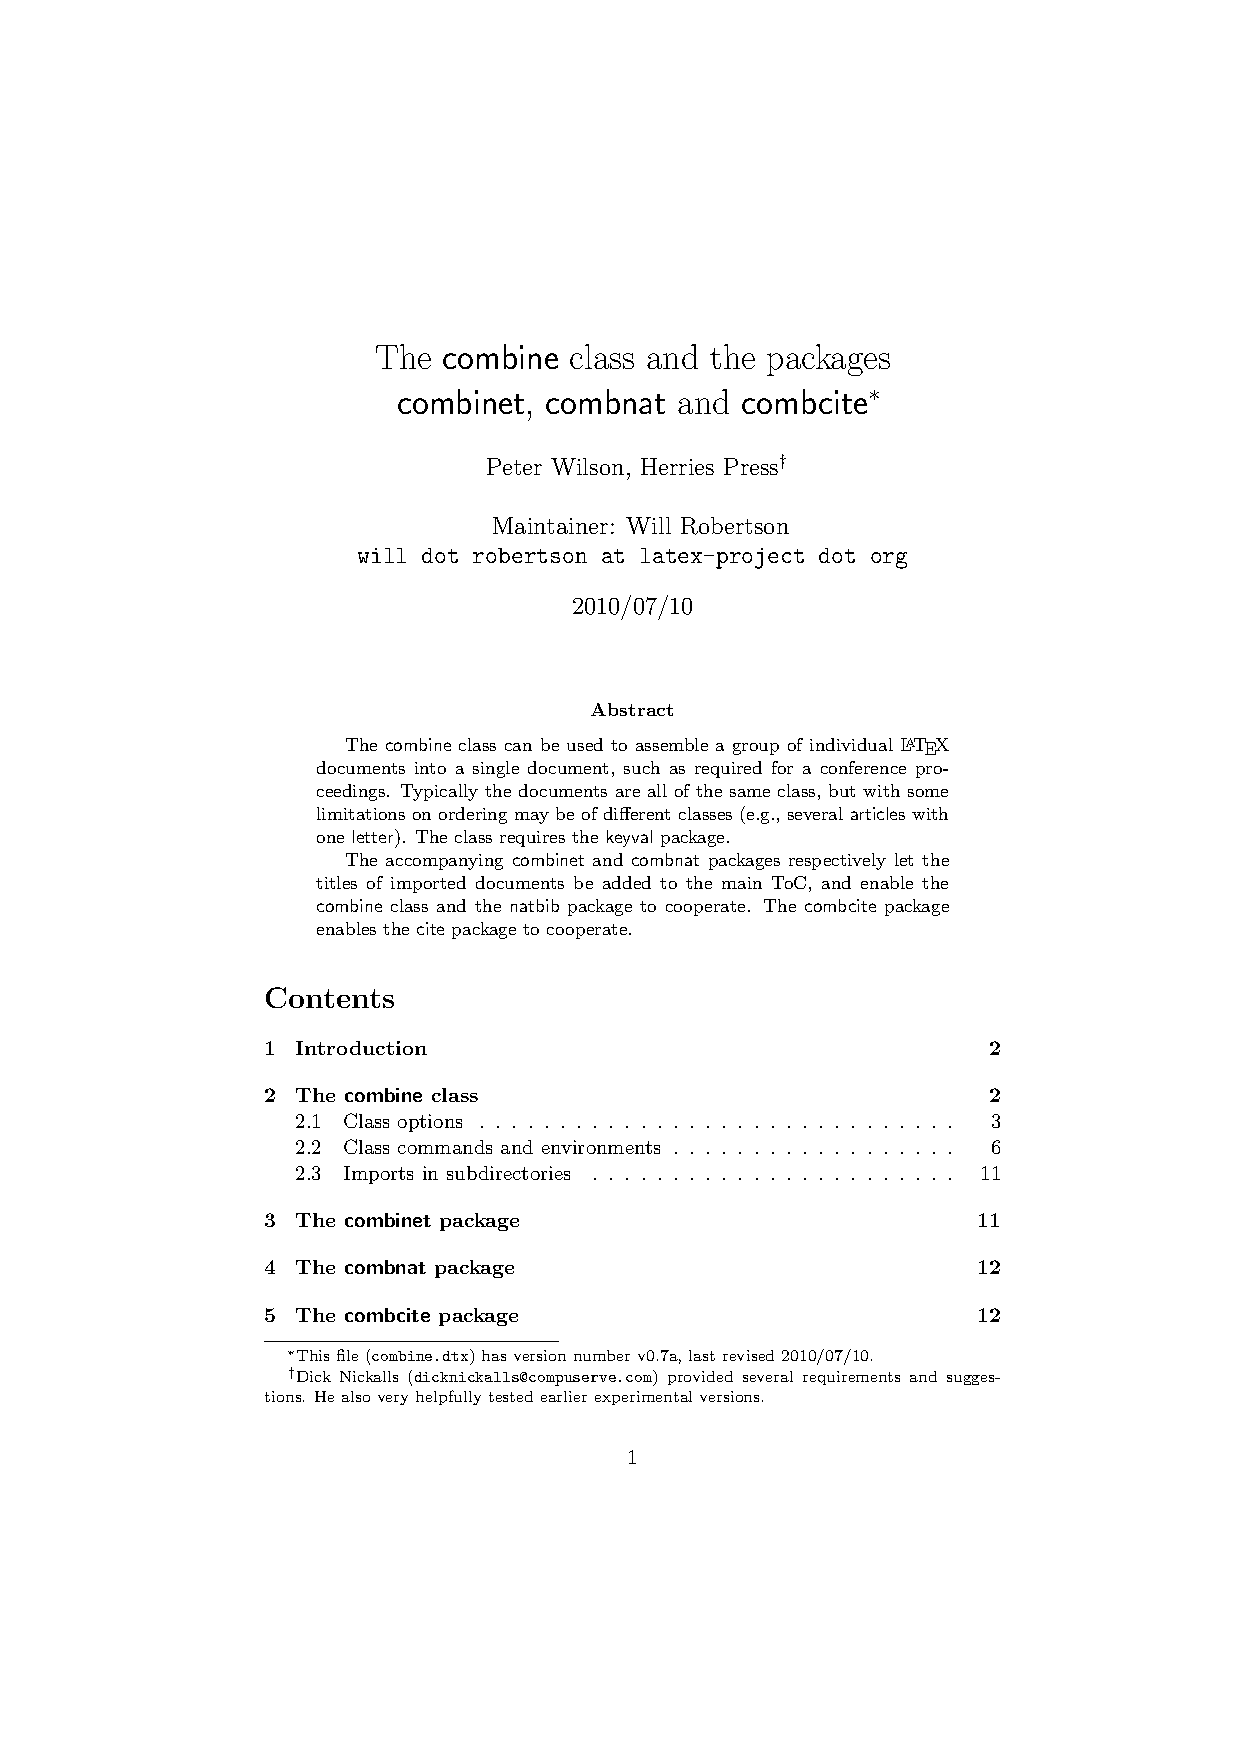
\includegraphics[width=.33\linewidth]{graphics/combine}
\caption{Combine Files into a Single PDF}\label{combine}
\end{center}
\end{figure}

The use of this feature is quite intuitive. Select the files you want to
include in your images file. Combine and save them to the appropriate
location. (\app{Acrobat} supports an enormous variety of file types,
includes PDF, JPG, PNG, GIF, etc.)

\subsubsection{Create and install a stamp file}\label{createinstall}

\textbf{Create.} To create a stamp file, take the sample file
\texttt{upres\_stamp.tex} and save it under a different name, say
\ameta{my\_stamps}\texttt{.tex}.  Bring your newly created stamp file into
your editor.
\begin{enumerate}
    \item Set the \cs{title} and \cs{author} of \ameta{my\_stamps} as
        desired. The \cs{title} will appear as a menu item of the
        \uif{Stamp} tool.
    \item Edit the argument of \cs{setStampPath} to point to the
        \texttt{image} file.
    \item Edit the argument of \cs{makeStamps}. There should be one
        token for each of the stamp images you are importing. Follow
        the formatting of the sample file.
    \item Compile \ameta{my\_stamps}\texttt{.tex}, convert to \textsf{PS}
    (using \app{dvips}), and distill using \app{Adobe
    Distiller}. This creates your stamp file
    \ameta{my\_stamps}\texttt{.pdf}.
\end{enumerate}

\textbf{Install.} After the stamp file is created, move it to the stamp
    folder, where \app{Acrobat} expects it to be. To find this location,
    start \app{Acrobat} and open the JavaScript Debugger Window
    (\texttt{Ctrl+J}/\texttt{Cmd+J}), and type in the following line of
    code,
\begin{Verbatim}[xleftmargin=20pt]
app.getPath("user","stamps");
\end{Verbatim}
Place your mouse cursor on this line and press
\texttt{Ctrl+Enter}/\texttt{Cmd+Enter} (or just use the \texttt{Enter} key on
the keypad). \app{Acrobat} will execute this line and return the path to the
user stamp folder. Navigate to this folder, and copy/move
\texttt{\ameta{my\_stamps}.pdf} to this folder.

Restart \app{Acrobat}, if all went as planned, your new stamps should be
listed in the menu listing of the \uif{Stamp} tool. Verify this. If successful,
they are ready for use!

\subsection{Using stamps with \textsf{annot\_pro}}

Earlier, on page~\pageref*{useannotpro}, the George Washington stamp was
used. The verbatim listing of that is given below.
\begin{Verbatim}[xleftmargin=20pt]
\annotpro[subject={AcroTeX makes stamps},title={D. P. Story},
type=stamp,name=\#George Washington]{You can use your
stamps through the user interface of Acrobat, or reference
them with the annot\_pro package!\n\n So says George
Washington!}
\end{Verbatim}
Note that the value of the \texttt{name} key is specified as \texttt{\#George
Washington}, not simply as \texttt{George Washington}. Custom stamp names
require their name be prefixed with a \texttt{\#}. The \pkg{mkstmp\_pro}
package automatically inserts the required prefix, but
\pkg{annot\_pro} does not.

See the documentation of \pkg{annot\_pro} for more details on how to use
the \cs{annotpro} command.

\section{The \texorpdfstring{\pkg{aeb\_dad}}{aeb\_dad} Package}

When \app{Adobe Reader XI} was released with its full support for comments
(and saving form fields), I saw this opened up possibilities for using
dragging and dropping stamps (DAD). Suppose you had a series of stamps,
and a series of push buttons. Each button is associated with one of the
stamps, but which one?  The user, even using \app{ARXI}, drags and drops a
stamp onto one of the push buttons. The underlying JavaScript determines
whether it was the right choice, if not, the stamp is returned to its
starting position. Below is the example demonstrated in
\texttt{dd\_uspres.tex}, the demo file for this package.

\begin{center}
{\large\bfseries DAD Matching (Game)}\medskip
\ddDimens
{%
    iconwidth=1in*\ratio{8bp}{10bp},iconheight=1.5in*\ratio{8bp}{10bp},
    targetwidth=1in*\ratio{8bp}{10bp},targetheight=1.5in*\ratio{8bp}{10bp}
}
\ddTargetFmt{\sffamily\small\bfseries}
\initDDGame{Presidents}

\ddGameIcon{George Washington}\quad
\ddGameIcon{John Adams}\quad
\ddGameIcon{Thomas Jefferson}\quad
\ddGameIcon{James Madison}\quad
\ddGameIcon{John Quincy Adams}

\medskip

\ddTargetOfIcon{John Quincy Adams}{John Quincy Adams}\quad
\ddTargetOfIcon{Thomas Jefferson}{Thomas Jefferson}\quad
\ddTargetOfIcon{James Madison}{James Madison}\quad
\ddTargetOfIcon{George Washington}{George Washington}\quad
\ddTargetOfIcon{John Adams}{John Adams}

\medskip

\ddReset
\end{center}
Drag and drop the image of each President onto the corresponding
rectangular region. Use your little gray cells, I am watching.

\textbf{\textcolor{red}{Important:}} Adobe has dropped its support for
online commenting, as a result, DAD Matching does not work from within a
browser. The user should download the file and view with \textsf{Adobe Reader
XI} (or later), or with the \textsf{Acrobat} application.

\subsection{Requirements and Installation}

The \pkg{aeb\_dad} package requires \pkg{annot\_pro} dated 2012/11/10 or later.

As for the installation of \pkg{aeb\_dad}, if not automatically
installed by a {\TeX} system, just copy \texttt{{aeb\_dad}.sty} into a
folder named \texttt{aeb\_dad}. If appropriate, refresh the filename
database of your {\TeX} system.

\subparagraph*{Examples and Documentation.} Unzip \texttt{mkstmpdad.zip}
anywhere you want, outside the {\LaTeX} search path. The \textsf{ZIP} file will
create a folder named \texttt{mkstmpdad}, containing program files, and
folders \texttt{doc} and \texttt{examples}.

\subsection{Testing the system}

The example file for this package is \texttt{dd\_upres.tex}. Assuming you
have installed and tested the Presidential stamps as per the instructions
in the section titled \mlNameref{createinstall}, you are ready to compile
the example file. After you compile, convert to \textsf{PS}, and distill
using \app{Adobe Distiller}, you get the PDF file, \texttt{dd\_upres.pdf}.
\emph{Don't forget to save the file}, this also saves the JavaScript that is
imported into the document.

The behavior of the stamps and push buttons in the file
\texttt{dd\_upres.pdf} is the same as the Presidents drag and drop
demonstration seen on the previous page.

\subsection{The details}

Let's look at the verbatim listing of \texttt{dd\_upres.tex}.

\def\Wdth{3.2in}
\hspace*{-62.5pt}\begin{minipage}[t]{\Wdth}\kern0pt
\begin{Verbatim}[numbers=left,xleftmargin=20pt,fontsize=\small]
\initDDGame{Presidents}

\ddDimens{%
    iconwidth=1in,iconheight=1.5in,
    targetwidth=1in,targetheight=1.5in}

\ddGameIcon{George Washington}\quad
...
\ddGameIcon{John Quincy Adams}

\ddTargetOfIcon{John Quincy Adams}
    {John Quincy Adams}\quad
...
\ddTargetOfIcon{George Washington}
    {George Washington}\quad
...
\ddReset
\end{Verbatim}
\end{minipage}\hfill
\begin{minipage}[t]{\linewidth+62.5pt-\Wdth-20pt}\kern0pt
\cs{initDDGame} initializes the DAD game, each game must have a unique
name.\vskip6pt
\cs{ddDimens} sets up the dimensions of the stamps and the push buttons.
\vskip6pt
\cs{ddGameIcon} is a command that sets up the positioning of the stamps,
the argument of this command is the \textit{name} of the stamp to be used.
\vskip6pt
\cs{ddTargetOfIcon} is a comment that creates a push button that is a
target of one of the stamps. The first argument is the \textit{name} of
the stamp, the second is the caption that appears beneath the push button.
\vskip6pt
\cs{ddReset} is a reset button. It puts the stamps back into their initial
positions, and returns the push buttons to their original appearance.
\end{minipage}
\par\medskip\noindent
The details follow in the order they appear in the document.

\subsubsection{Commands of \texorpdfstring{\pkg{aeb\_dad}}{aeb\_dad}}

In this section, several commands are presented; these are used to define and design your
DAD Game.
$$
    \fbox{\parbox{4in}{\textbf{A DAD Game must appear on a single page.} You must
    design the `game board' to appear in one page, that might require
    making the stamps and targets smaller, or the page width wider.}}
$$
Begin by declaring the game title of the DAD Game.
\bVerb\takeMeasure{\string\initDDGame\darg{\ameta{title}}}
\begin{minipage}{\bxSize}
\begin{Verbatim}[frame=single,commandchars=!()]
\initDDGame{!ameta(title)}
\end{Verbatim}
\end{minipage}\eVerb
The \cs{initDDGame} command must appear on the same page on which the
stamps and push buttons appear. The argument \meta{title} is the title of
the DAD game; typically, it should follow the same rules as a JavaScript
variable, because it forms the base name of the push buttons and the reset
button. \cs{initDDGame} defines a page option action that sorts through
the stamps on the page for the ones that belong to the DAD Matching Game
with a name of \meta{title} and places them in an array.

\bVerb\takeMeasure{\string\ddDimens\darg{\ameta{KV-pairs}}}
\begin{minipage}{\bxSize}
\begin{Verbatim}[frame=single,commandchars=!()]
\ddDimens{!ameta(KV-pairs)}
\end{Verbatim}
\end{minipage}\eVerb
The key-values are,
\begin{itemize}
\item \texttt{iconwidth=\ameta{width}} is the width allotted to the icon
(stamp). The default value is \cs{defaultStampWidth}, defined in
\pkg{annot\_pro} as 50bp.
\item \texttt{iconheight=\ameta{height}} is the height allotted to the icon
(stamp). The default value is \cs{defaultStampHeight}, defined in
\pkg{annot\_pro} as 50bp.
\item \texttt{targetwidth=\ameta{width}} is the width of the target push
button. The default value is 1.25in, as set by \pkg{aeb\_dad}.
\item \texttt{targetheight=\ameta{height}} is the height of the target push
button. The default value is 1.25in, as set by \pkg{aeb\_dad}.
\end{itemize}

\bVerb\takeMeasure{\string\ddGameIcon\darg{\ameta{icon\_name}}}
\begin{minipage}{\bxSize}
\begin{Verbatim}[frame=single,commandchars=!()]
\ddGameIcon{!ameta(icon_name)}
\end{Verbatim}
\end{minipage}\eVerb
This is the command that places a stamp with name of \ameta{icon\_name}.
Use this command repeatedly with, of course, different names. Arrange
them on the page as desired.

\bVerb\takeMeasure{\string\ddTargetOfIcon\darg{\ameta{icon\_name}}\darg{\ameta{caption}}}
\begin{minipage}{\bxSize}
\begin{Verbatim}[frame=single,commandchars=!()]
\ddTargetOfIcon{!ameta(icon_name)}{!ameta(caption)}
\end{Verbatim}
\end{minipage}\eVerb
This command creates a target push button. There must be one
\cs{ddTargetOfIcon} for each \cs{ddGameIcon}. The first argument,
\ameta{icon\_name} must match one and only one \ameta{icon\_name} argument
of \cs{ddGameIcon}. (There must be a one-to-one correspondence between
stamps and push buttons.) The second argument \ameta{caption} is a short
caption that appears at the bottom of the button. This caption should be
descriptive on the icon (stamp) that it matches with.

\pkg{aeb\_dad} defines two other commands that relate to \cs{ddTargetOfIcon}, these
are \cs{ddTargetCaption} and \cs{ddTargetFmt}, the default definitions of which
are seen below.
\begin{Verbatim}[xleftmargin=20pt,commandchars=!()]
\newcommand{\ddTargetCaption}[1]{\\[3pt]%
    \parbox[t]{\linewidth}{\centering\ddm@targetfmt#1}}
\newcommand{\ddTargetFmt}[1]{\def\ddm@targetfmt{#1}}
\ddTargetFmt{}
\end{Verbatim}
\cs{ddTargetCaption} sets the caption in a \cs{parbox} that is 3pt beneath
the button. The command \cs{ddm@targetfmt} is a formatting command, it is
defined by \cs{ddTargetFmt}. Use the command \cs{ddTargetFmt} to set the
formatting (or styling) of the captions, it takes one argument which is
passed to the tex stream prior to the caption. For example, for the
President Stamp game appearing on page~\pageref{useannotpro}, we  declared
\begin{Verbatim}[xleftmargin=20pt,commandchars=!()]
\ddTargetFmt{\sffamily\small\bfseries}
\end{Verbatim}
The default is \verb!\ddTargetFmt{}!, no styling.

\bVerb\takeMeasure{\string\ddReset\darg{\ameta{title}}}
\begin{minipage}{\bxSize}
\begin{Verbatim}[frame=single,commandchars=!()]
\ddReset[!ameta(title)]
\end{Verbatim}
\end{minipage}\eVerb
The \cs{ddReset} button restores the most recently defined DAD Matching
Game to its original state. If, for some reason, the most recent one  is
not the one you want reset, use the optional argument \meta{title} to pass
the title of the game you want reset.

It is recommended that the reset button be always on the screen when the user
is matching icons. The game executes a \texttt{Field.setFocus()} method to
take the focus off the stamps when they are dropped. The focus goes on the
reset button. If the reset button is out of the user's viewing, \app{AA} or
\app{AR} will scroll the page to place the reset button in the (middle of
the) viewing area. This would not be a good experience for the user.  For
documents that are screen size, placement below the game is probably
acceptable; for paper size pages, placement of the reset button between the
row of stamps and the row of target buttons may work.


\subsubsection{Customizing the JavaScript}

When a correct matching is made, the JavaScript function
\texttt{ddCorrectAction()} is executed; and when an incorrect matching is
made, \texttt{ddWrongAction()}. These two functions simply
place an alert box on the screen with the message ``Right!'' or ``Wrong'',
depending. These two messages, as well as  three others, are
defined below.
\begin{Verbatim}[xleftmargin=20pt]
\newcommand{\ddRightMsg}{"Right!"}
\newcommand{\ddWrongMsg}{"Wrong!"}
\newcommand{\ddDragOnlyOne}{"Drag one icon at a time"}
\newcommand{\ddExternalMsg}{%
    "Drag and Drop of icons does not work in a browser. "
        + "Save this file to your computer and view it in "
        + "Adobe Reader XI or later, or in the "
        + Acrobat application."
}
\newcommand{\ddBadAppMsg}{%
    "Any version of Adobe Acrobat, "
        +"or Adobe Reader XI is required!"
}
\end{Verbatim}
These may be redefined to other messages as desired.

The two functions \texttt{ddCorrectAction()} and \texttt{ddWrongAction()}
first test for the presence of \texttt{ddCustomCorrectAction()} and
\texttt{ddCustomWrongAction()}. If either one (or both) are defined, then
these functions will be executed. The two JavaScript functions,
then, are hooks into the system to modify how the game reacts to being
right or wrong. See the second demo file \texttt{dd\_uspres\_custom.tex}
for an example. The verbatim listing of the definitions of custom
functions are given and discussed below. This example is just one of many
possible definitions.


\begin{Verbatim}[numbers=left,xleftmargin=20pt,fontsize=\small]
\begin{insDLJS}{dd}{Custom Notifications}
var oAlertTitle=new Object();
oAlertTitle["Presidents"] = "The Presidents of the United States";
function ddCustomCorrectAction(event,ddName) {
    app.alert({cMsg: "That's right! Out of sight! ("+ddStats.nCorrect
        +" out of "+ddStats.nTries+")",
        nIcon: 3, cTitle: "AeB Drag and Drop: "
            +oAlertTitle[ddName]});
}
function ddCustomWrongAction(event,ddName) {
    app.alert({cMsg: "Ding, Dong, that is Wrong! ("+ddStats.nCorrect
        +" out of "+ddStats.nTries+")",
        nIcon: 0, cTitle: "AeB Drag and Drop: "
            +oAlertTitle[ddName]});
}
\end{Verbatim}

\begin{itemize}
    \item Lines~(2) \&~(3) show how to get a custom title on the alert
    box, optional, just an idea.
    \item Lines~(4)--(14) is the custom handler when the user has a
    correct matching.
    \begin{itemize}
        \item There is a built in counter that tracks the number correct
        and the number of attempts. The counter array is shown in
        lines~(6) \&~(7). The first one, line~(6), keeps track of the
        number correct, and the other one, line~(7), is the total
        attempts.

        The reset button \cs{ddReset} resets the counters to zero again.

        \item Lines~(10)--(13) is a custom alert box, that would
        say, for example, ``That's Right! Out of sight! (2 out of 5)''.
    \end{itemize}
    \item Lines~(15)--(24) show the definition of
    \texttt{ddCustomWrongAction()}. It has a similar structure, but does
    not increment the number correct.
\end{itemize}
There are other ideas that come to mind.  You can create a text field, and
define your custom functions to write the score to it. Within the reset
JavaScript function \texttt{resetDDM()}, a check is made for the presence
of a function named \texttt{ddCustomResetAction()}; if it exists, it is
executed as \texttt{ddCustomResetAction(page,ddName)}, where \texttt{page}
is the page number on which the game resides, and \texttt{ddName} is the
title of the game. You can use, for example, to then reset any text field
you define to hold the score.

\subsection{Additional Examples}

Additional examples are posted on the
\href{http://blog.acrotex.net}{\AcroTeX{} Blog Site}, these can be conveniently found
under the tag
\href{http://www.acrotex.net/blog/?tag=mkstmpdad}{\emph{mkstmpdad}}.

\bigskip\noindent
Now, I simply must get back to my retirement. \dps

\end{document}
